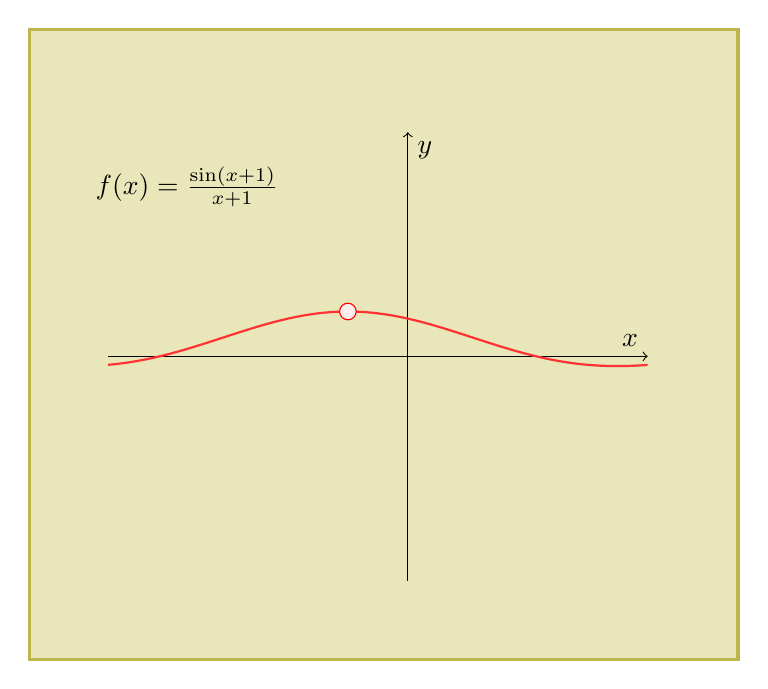
\begin{tikzpicture}
  \draw[draw = olive!60, fill = olive!20, very thick]
    (-1, -1) rectangle (8, 7);

  \begin{axis}[
    xmin = -5,
    xmax = 4,
    ymin = -5,
    ymax = 5,
    axis x line = middle,
    axis y line = middle,
    xlabel = \(x\),
    ylabel = \(y\),
    axis line style = {->},
    ticks = none,
    smooth,
  ]
    \addplot[thick, red!80, domain = -5 : -1.01]
      {sin(deg(x + 1)) / (x + 1)};
    \addplot[thick, red!80, domain = -0.99 : 4]
      {sin(deg(x + 1)) / (x + 1)};

    \addplot[
      mark = *,
      mark options = {
        scale = 1.5,
        fill = white!70!pink,
        draw = red,
      },
    ] coordinates {(-1, 1)};

  \end{axis}

  \draw (1, 5) node {\(\display{f(x) = \frac{\sin (x + 1)}{x + 1}}\)};

\end{tikzpicture}